\documentclass{chi-ext}

\copyrightinfo{
  Copyright is held by the author/owner(s).\\
  \emph{CHI 2012}, May 5--10, 2012, Austin, TX, USA.\\
  ACM xxx-x-xxxx-xxxx-x/xx/xx.\\
}

\title{Tangible Tube}

\numberofauthors{3}
% Notice how author names are alternately typesetted to appear ordered in 2-column format;
% i.e., the first 4 autors on the first column and the other 4 auhors on the second column.
% Actually, it's up to you to strictly adhere to this author notation.
\author{
  \alignauthor{
    \textbf{Hilfi Alkaff}\\
    \affaddr{University of California, Berkeley}\\
    \affaddr{Berkeley, CA 94720 USA}\\
    \email{hilfia@eecs.berkeley.edu}
  }
  \alignauthor{
    \textbf{Kimiko Ryokai}\\
    \affaddr{University of California, Berkeley}\\
    \affaddr{Berkeley, CA 94720 USA}\\
    \email{kimiko@ischool.berkeley.edu}
  }
  \vfil
  \alignauthor{
    \textbf{Albert Tjoeng}\\
    \affaddr{University of California, Berkeley}\\
    \affaddr{Berkeley, CA 94720 USA}\\
    \email{albert\_tjoeng@berkeley.edu}
  }
  \vfil
  \alignauthor{
    \textbf{Victor Tjhia}\\
    \affaddr{University of California, Berkeley}\\
    \affaddr{Berkeley, CA 94720 USA}\\
    \email{victor.tjhia@berkeley.edu}
  }
  \vfil
  \alignauthor{
    \textbf{Alyssa Novelia}\\
    \affaddr{University of California, Berkeley}\\
    \affaddr{Berkeley, CA 94720 USA}\\
    \email{a.novelia@berkeley.edu}
  }
}

% Paper metadata (use plain text, for PDF inclusion and later re-using, if desired)
\def\plaintitle{Tangible Tube}
\def\plainauthor{Hilfi Alkaff, Albert Tjoeng, Victor Tjhia}
\def\plainkeywords{Tangible User Interfaces, Interaction Design, Children, Entertainment, User Experience, User Interface Design, Usability Research}
\def\plaingeneralterms{Design, Experimentation}


\hypersetup{
  pdftitle={\plaintitle},
  pdfauthor={\plainauthor},
  pdfkeywords={\plainkeywords},
  pdfsubject={\plaingeneralterms},
}

\usepackage{graphicx} % for EPS use the graphics package instead
\usepackage{balance}  % useful for balancing the last columns
\usepackage{xspace}

\newcommand{\tube}{\textsf{Tangible Tube}\xspace}
\newcommand{\eg}{\emph{e.g.,}}
\newcommand{\ie}{\emph{i.e.,}}
\newcommand{\TODO}{\textbf{TODO:\newline}}

\begin{document}

\maketitle

\begin{abstract}

\tube is a device that invites users to play in a completely unprecedented form of interactions. Instead of utilizing traditional devices such as keyboards, mouse, joysticks and wii remote controls that challenges users on how swift and composed their fingers' movements are, \tube challenges users to play games using a tube that they will control through breathing and moving their body.

\end{abstract}



\keywords{\plainkeywords}

\category{H.5.m}{Information interfaces and presentation (e.g., HCI)}{User Interfaces, user centered design}.

\terms{\plaingeneralterms}

\section{Introduction}\label{sec:intro}

There has been a few works that explores user interface system that utilizes breathing.

\textbf{Tooka~\cite{tooka}:} This is a tube which acts like a musical instrument. Each player can blow from the opposite end of the tube and produce the sound collaboratively using their tongues and lungs, and by pressing the buttons. The main difference of this tube and our \tube is in the output produced. While the Tooka focused more on producing sound as a musical instrument, our tube is simply a device used for interaction between users and our software which focus primarily on gaming. Our tube is also capable for more different user interaction as it detects rotation and 2-D movement while the Tooka seems to support only pressure modulation and button inputs.

\textbf{BLUI~\cite{blui}:} BLUI (Low-cost Localized Blowable User Interface) is a hands-free interaction between user and computer by blowing the computer screen to control the interactive application. Both our systems seem to be able to support similar application; however BLUI supports blowing directly to the computer screen while \tube uses a tube as a device for interaction.

\textbf{The Pipe~\cite{thepipe}:} This is a music input device using breath pressure as control input. Pipe that is used in this projects uses similar sensors that are used in our tube such as accelerometer and force sensing sensor. The main difference is the output; The Pipe focuses on building a musical instrument while \tube acts as a device for users to control out application.

\TODO
- Traditional entertainment software: PS, nintendo and newer game console: wii

Video games have become one of the most popular entertainments for most children and teenager, even young adults. Console such as Nintendo and Sony PlayStation were considered as the pioneers that popularize video games in our society. However, most video games only require the users to press the buttons and the result will be displayed on the screen, built-in screen or TV. There is no other interface between the users and the system besides pressing the button in the handheld. On 2006, Nintendo released Wii, a console that uses a remote controller to detect users’ movement in 3-D. This console introduced a new and interactive way of playing video games because it involves user moving the remote instead of only pressing the buttons. 

In this paper, we present \tube, an interactive and tangible system that employs breathing control. We will discuss the features and possibilities of \tube becoming a new system to use an interactive applications and games.

\section{Implementation}\label{sec:impl}

The \tube system has two components; the tube itself and the screen. The tube is attached to an acrylic enclosure that houses a small Force-Sensing Resistor (FSR) and Inertial Measurement Units (IMU) that possesses 5 degree of freedom. The IMU captures the 3-dimensional motions of the tube and translate it into 2-dimensional movement in the screen. Additionally, it also records the angle in which the tube is rotated and how fast it is rotating. With the FSR integrated in the tube, how hard the user breathe into the tube is also captured. All of these informations will then be passed into arduino which will be read by a processing module.

\begin{figure}
  \centering
  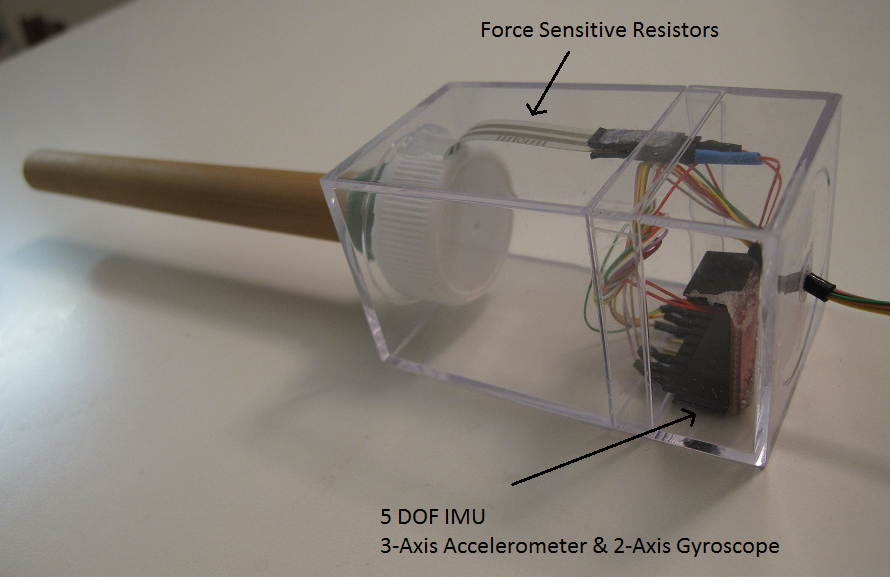
\includegraphics[width=\linewidth]{./figs/impl1.png}
  \caption{The Tangible Tube with all the sensors.}
  \label{fig:impl1}
\end{figure}


We have developed two applications to demonstrate the interactivity of our \tube. The applications that we developed are written in processing since it provides a smooth interface with arduino while boasting numerous easy-to-use graphical functions. Making existing processing applications to work with our \tube require very minimal changes to the code base since we have made the interface to the hardware to be very simple and generic.

% \subsection{Painting}
===== Painting picture here ======

Our first application is a painting application program. In this application, the user will be able to paint by blowing into the tube and the harder the user blows, the thicker the color is. Changing the color of the paint is achieved by rotating the tube. We implement the paint to be brush-like and the color will disappear after a while to make it more like painting with a real brush.


% \subsection{Shooting Game}
===== Balloon picture here =======

The picture above shows our balloon popping game. In this game, the user is required to pass through a set of levels by shooting down balloons that randomly appear in the screen. This is done by moving the pointer to where the balloons are and blow into the tube. The game consists of two levels: stage 1 and stage 2. In the first stage, the pointer and balloons color are always black so that users don’t have to rotate the tube to match the color. This stage is intended to familiarize the users with the basic concept on how to move the tube to control the pointer and use it to pop a balloon. The pointer is shaped like a circle and whenever the users blow the tube, the pointer will become a like a flower petal which size is determined by how hard the user blow. Every time a balloon is popped, the user will receive 1 point. After scoring a few points in the first stage, we take the users to stage 2 where the balloons are randomly generated with red, green, or blue color and the users will have to rotate the tube to change color of the pointer so that they can pop the balloon. When the game ends, users can simply blow the tube harder and it will take them back to stage 1. 



\TODO
- Pictures \newline
- More details


\section{Design}\label{sec:design}

In this section, we describe the points that we took into account when designing our tube. Firstly, we would like to make sure that the users will immediately understand how to use \tube at the first sight of it without any instruction given to them. In order to accomplish this, we designed the mouth piece of the device similar to a blowgun so that the users will understand immediately that the tube is meant for blowing. We have also attached a colored circle in front of the mouth piece to inform the users that rotating the device will change the output color accordingly.

\section{Evaluation}\label{sec:eval}
In order to measure how interactive our \tube is, we developed our application to be able to take inputs from traditional input devices (\ie mouse and keyboard) and our \tube. For instance, in the shooting game applications the users will be able shoot down the balloons by clicking on the mouse and to match the color of the aballoons with the mouse pointer that the user is controlling, the user will need to press some keys in the keyboard.

After describing to our participants how our \tube works, the participants tried out the applications that we have developed both with and mouse and keyboard and with \tube as the input device.

\begin{figure}
  \centering
  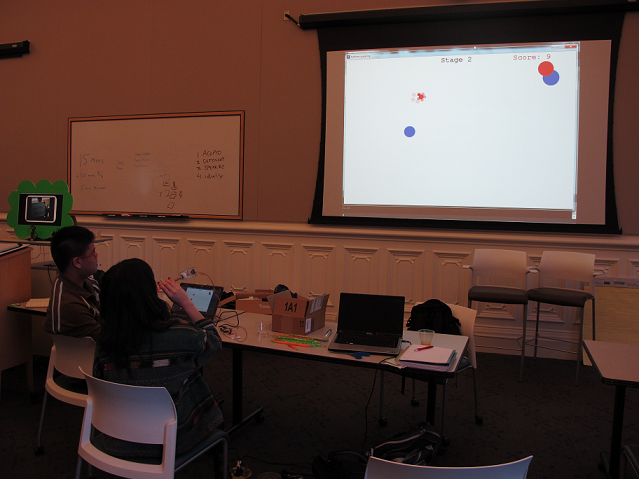
\includegraphics[width=\linewidth]{./figs/impl2.png}
  \caption{The participants trying out The Tangible Tube during a project showcase on December 7th 2011 at UC Berkeley campus.}
  \label{fig:impl2}
\end{figure}

The first thing that the testers do when trying out the /tube was figuring how to control the small pointer on the screen. Since there is feedback from the screen to show where the pointer is, the testers adapt to the system naturally and in no time successfully playing with /tube. The challenging part is when you have to match the color with the color of the balloon by rotating the tube. This is when the unique interaction with the system starts. The testers see that they cannot pop the balloon without matching the colors and start to rotate while blowing the tube. 


\TODO
- Pictures \newline
- Describe the experience of the testers. \newline
- Evaluate how \tube is representative for games like balloon popping.

\section{Discussions and Future Work}\label{sec:fut-work}
In the future, we would like to explore on how well \tube works in a collaborative setting. For instance, in the shooting game that we developed, we could extend the game so that two people will compete to get a higher score or collaborate to shoot down a number of balloons under limited time. We believe that our \tube will be much more interactive if this is implemented.

Following up our previous point, making \tube wireless is essential to maximize the user experience. In our current prototype, our \tube is wired to the laptop. In this case, the users will be constrained at how long the wire connecting the tube to the computer is and could not move as freely when using the applications. Under group setting, this problem is exacerbated since multiple users could now collided with each other due to space constraints and this will definitely detriment the user experience.

Instead of utilizing computer screen as the output of our \tube, we believe that it will be best if it is displayed on a standalone screen such as a television screen so that the \tube system will feel more natural to the user and not just "another computer application".

Instead of utilizing computer screen as the output of our \tube, we believe that it will be best if it is displayed on an interactive output such as a table tops so that the \tube system will have more natural user interaction and not just "another computer application".

Last but not least, in the hardware side, we also need to smoothen the reading that we get from the accelerometers and gyroscopes in order to maximize user experience.


\section{Conclusion}\label{sec:conc}

In this paper, we have reported on the design and the first prototype of a tangible user interface that revolves around breathing actions of the users instead of one that utilizes keyboard or joysticks presses. We believe that this invites our users into a realm of interactions that they have not explored yet before. The amusement of people who tested our \tube, even in the simple games that we developed, have confirmed our success and encouraged us to explore this further.

This project is still ongoing and will continue to develop. From the feedbacks given by the testers, we believe that we can improve the systems greatly by adding a few more important features as mentioned in the future work section.

\section{Acknowledgment}\label{sec:ack}
We would like to thank Kimiko Ryokai, Han-Shue Tan, Jihua Huang, and George Anwar for their numerous suggestions that improved this project a lot.


\balance
\bibliographystyle{abbrv}
\bibliography{main}

\end{document}
